% Sample file on how to use subfiles.
\documentclass[ExampleMasters.tex]{subfiles}

\begin{document}
\clearpage


\chapter{Software Architecture (8 Seiten)}
\label{chap:software_setup}

\section{Functionality architecture}
\label{sec:func_architecture}

\begin{itemize}
	\item describe VTT funct. artchitecture
	\item make and insert sketch for (1)
	\item outline which software system correspondes to what
	\item differentiate between HiL, Bench and track
	
\end{itemize}
\begin{figure}[h]
\centering
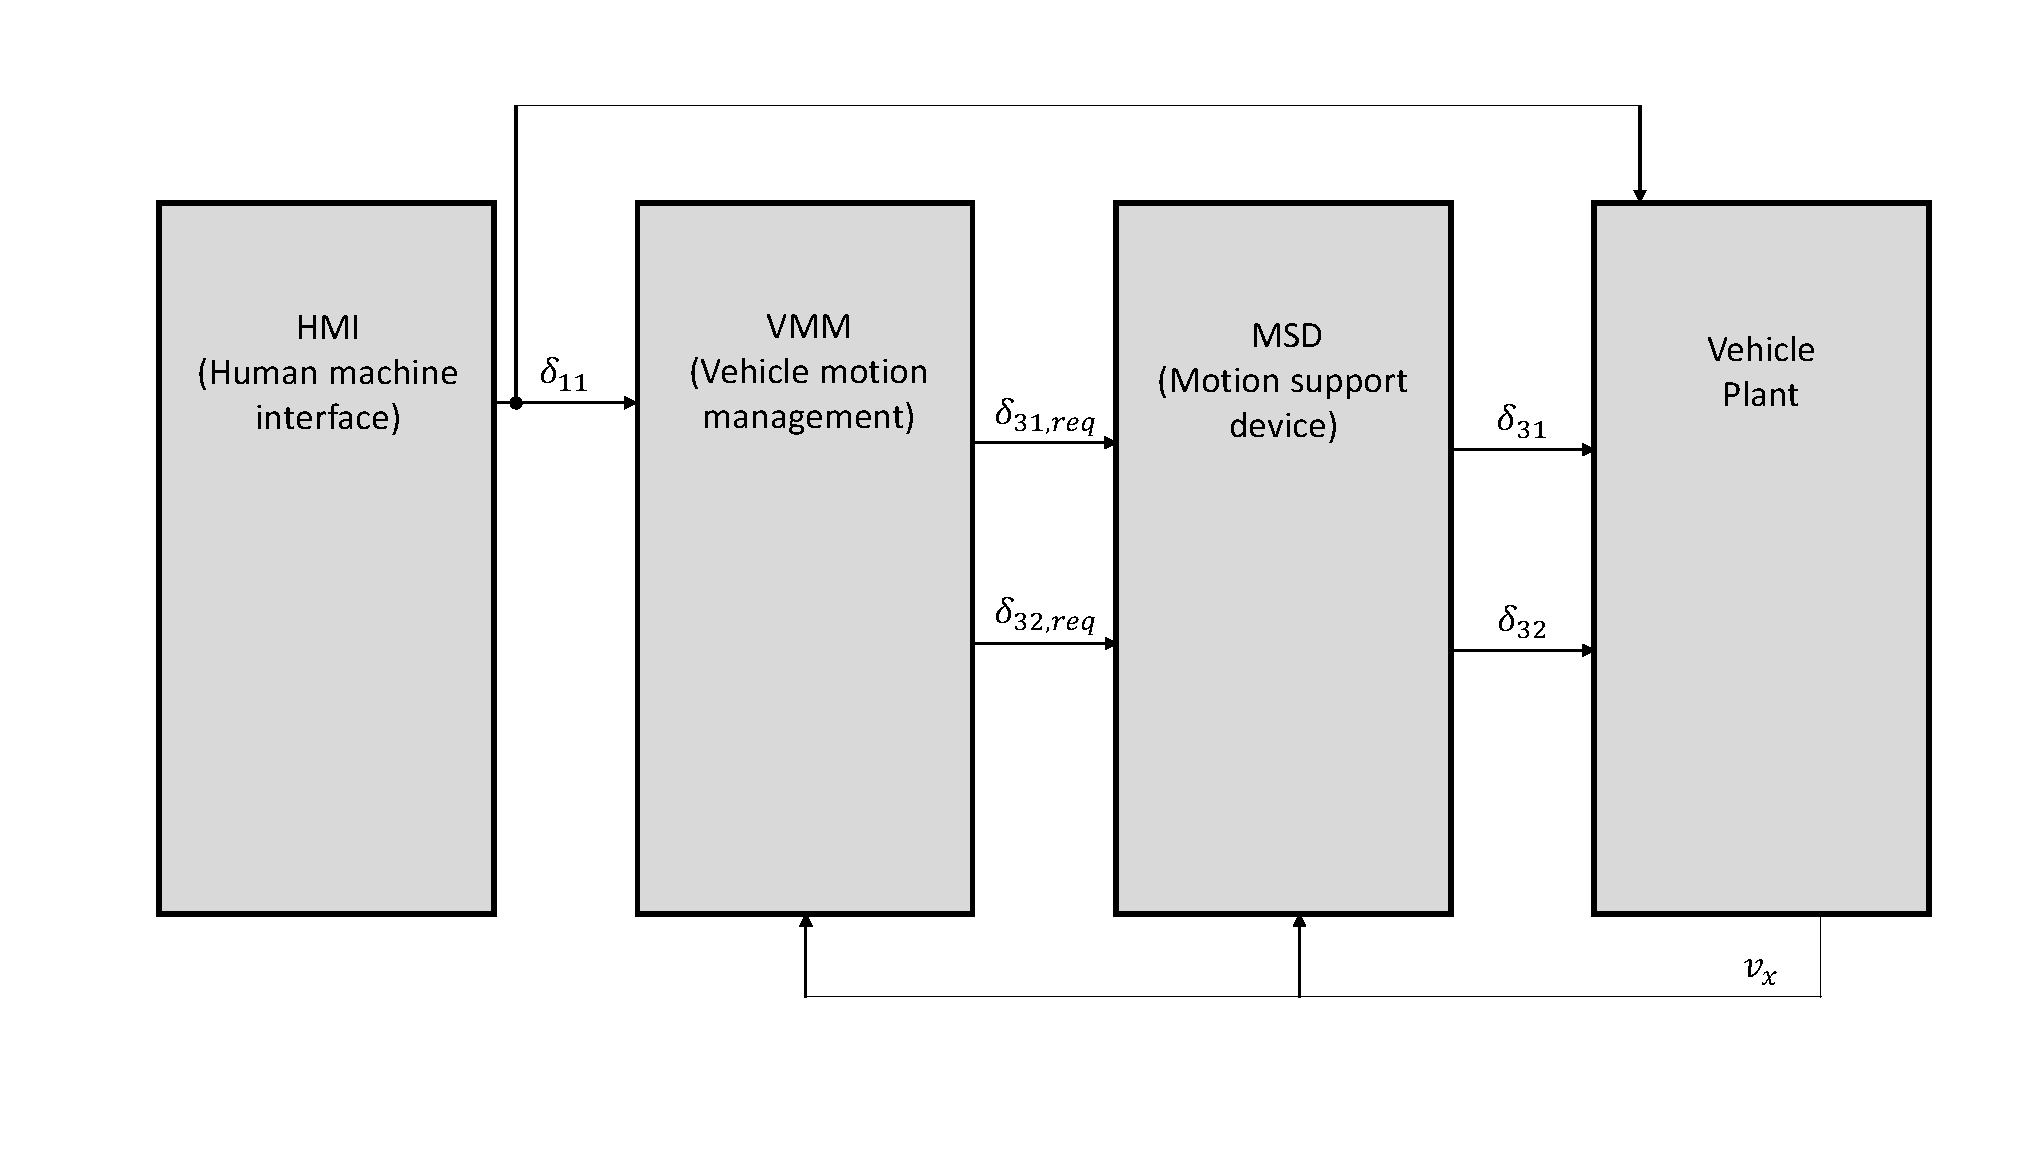
\includegraphics[width=1\linewidth]{figures/functionality_architecture}

\caption{Functionality Architecture}
\label{fig:funct_architecture}
\end{figure}

\section{Matlab/Simulink environment}
\label{sec:matlab}

%%\subsection{FMI toolbox}



\subsection{dSpace RTI-blockset}
The dSpace RTI-Blockset (Real-time interface) is a plug-in for MATLAB/Simulink that allows you to connect a simulink-model to the different inputs and outputs of the MABII. There are RTI-blocks for CAN, Ethernet, LIN, FPGA and the analog and digital outputs of the MABII.
In this project the RTI CAN MultiMessage and the RTI Ethernet (UDP) Blocksets were used.\\ 
\subsubsection{RTI CAN MultiMessage Blockset}
The RTI CAN MultiMessage blocks establish an interface between the physical CAN-Buses of the MABII and the simulink-model running on the MABII. There are four different blocks in this blockset: 

In the "GeneralSetup" block the paths of the model root and the destination folder for generated files are set. 

In the "ControllerSetup" block first the name of the controller has to be set. After that the physical CAN-Bus, that should be used, is set by choosing a module number and a controller number. How the module- and controller numbers have to be set for the different CAN-buses of the MABII is shown in \ref{tab:CAN-layout}.
\begin{table}[h]
	\centering
	\caption{CAN-layout MABII}
	\label{tab:CAN-layout}
	\begin{tabular}{c|c|c|c|c|}
		CAN   & Module number & Controller number & ZIF-Pin CAN-High & ZIF-Pin CAN-Low  \\ \hline
		CAN1     &       1 & 1  & c2 & c3         \\
		CAN2   &      1 & 2  & b2 & b3    \\
		CAN3 &      2 & 1 & B2 & B3        \\
		CAN4& 2 & 2 & A2 & A3  \\
		CAN5& 3 & 1 & P2 & P3 \\
		CAN6& 3 & 2 & N2 & N3 \\
	\end{tabular} \\
\end{table}

After setting the module- and controller number the identifier format has to be set to either standard or extended format, the transceiver type must be chosen between ISO11898-2 and ISO11898-6. ISO11898-2 is used for a high-speed medium access unit and ISO11989-6 for the selective wake-up functionality of a high-speed medium access unit. If needed, a termination resistance of 120 Ohms can be set in the block as well. As a last step the Baud rate of the CAN-bus has to be defined.


In the "Main Block" block a dbc-file is connected to one of the controller blocks, that were created before. A "ControllerSetup" block can only be connected to one "Main Block" at a time. When the dbc-file is loaded in the "Main Block", the different messages and signals that are specified in the dbc-file can be chosen as inputs and/or outputs of the "Main block". For signals that should be transmitted it has to be defined when they should be transmitted. There are different ways to specify this. One way is to set a cycle time in the simulink model, that determines with which frequency the signal is sent out. Another way is to use triggers that trigger the transmission every time a specific event happens. This can be set in the tab "Messages" under "Triggering".
\subsubsection{RTI Ethernet (UDP) Blockset}
The RTI Ethernet (UDP) Blockset was used for two purposes: On the one hand for the HIL-testing (see section \ref{sec:HIL}), on the other hand for the CAN-bus extension of the MABII (see section \ref{sec:can_bus_extension_software}). The RTI Ethernet (UDP) Blockset contains four different blocks:\\
The "Ethernet\_UDP\_SETUP" block consists of two pages. In the "Unit" page the main settings for the Ethernet are made. First the interface name has to be chosen. Then the board type has to be selected. There are two types of boards: "ETH Type 1" and "ECU Type 1 ETH". If the Ethernet cable is connected to the Ethernet port of the MABII, "ETH Type 1" has to be chosen. The module number, which has to be set in the next step, must be set to 1 since the used MABII only has one module.
After that, the local IP address has to be set.\\
On the options page of the setup block up to four different sockets can be enabled. For each socket a local port number, the remote ip address and the remote port number have to be set.\\
 
The "Ethernet\_UDP\_RX" block is used to receive data over Ethernet. To set up this block the board type, module number and socket number need to be set corresponding to the settings that were made in the "Ethernet UDP Setup" block. Furthermore the maximum message size can be defined. Outputs of this block are the received data, the message size and a status. The datatype of the received data is uint32. If the data wasn't transmitted as uint32 it needs to be decoded. In the demo for the Ethernet blocks a block called "DSDecode32" can be found. With this block the decoding can be done, by choosing the desired output data format. To get the single signals the output of that block just needs to be demuxed. If the data type of the transmitted data was already uint32 the signal can be demuxed right away.

The "Ethernet\_UDP\_TX" block is used to send data over Ethernet. This can be done in a similar way as for the receive block. The only difference is that in the transmit block additionally a send timeout can be set. The maximum message size must match the port width of the data that is send out. It can be calculated by:
\begin{equation}
data\ port\ width=(MaxMessageSize + 3) / 4
\end{equation}
The inputs to the transmit block are the data to transmit, the message size and a constant to enable the transmission. The data format of the data to transmit needs to be uint32. Similar to the receive block a so called "DSEncode" block can be found in the demo for this blockset. This block encodes muxed signals of different types in a way, that they can be transmitted with the transmit block. In the "DSEncode" block the data type of the different signals, that are put in the block, need to be specified.

The "Ethernet\_UDP\_INTERRUPT" can be used to make the hardware interrupts available as trigger sources.
\subsection{Virtual Truck Modelling Library}
\label{sec:VTM}
The Virtual Truck Modelling Library (VTM) is a computational framework used within Volvo Trucks to simulate the dynamic behaviours of trucks and combinations. As a library it extends Simulink, where maneuvers, track layout and the trucks kinematic and dynamic properties are linked together and then computed. This toolbox was used as a base for the simulation of the LVC including the dolly for this project. It is possible to run simulation offline with a predefined maneuver and a given environment as well online where these parameters are fed into the calculation live or as measurings from the real-world environment. For online use all relevant parameters and states can be accessed in Simulink or in case of execution on the MABII through ControlDesk as their respective representation of the Simulink variable. 

\subsection{CAN-bus extension}
\label{sec:can_bus_extension_software}

\begin{itemize}
	\item outline data diagram structure
	\item show limitations uf UDP (time, reliability, retrans)
	\item timestamping
	
	
\end{itemize}


\section{ControlDesk monitoring environment}
\label{sec:control_desk}
\subsection{Maneuver control}


\subsection{Monitoring and logging}
\begin{itemize}
	\item data-format
	\item frequency
	\item synchronizing over different CANs	
\end{itemize}


\section{Arduino IDE and applications}
\label{sec:arduino_applications}

The Arduino system provides an integrated development environment (IDE)  written in Java, providing cross-platform support. It is used to develop the code as well as compiling the code and subsequently uploading it into the microcontroller via the computers serial interface. Within the IDE it is also possible to load some of the officially supported libraries directly. It conveniently is possible to monitor the computer's serial interface as well, which is the most practical way to monitor and debug code that is executed on the Arduino. 

\begin{table}[h]
	\label{tab:list_of_arduino_libs}
	\begin{tabular}{lll}
		\textbf{Library name} & \textbf{Purpose}                                    & \textbf{Comment} \\
		LSM303                & read magnetometer on IMU via I2C                    &                \cite{lsm303_github}  \\
		L3G                   & read gyro \& accelerometer on IMU via I2C           &      
		\cite{l3g_github}            \\
		UIPethernet           &     control ENC28J60 via SPI                                                &             \cite{uip_ethernet_github}     \\
		TinyGPSPlus           & acquire and parse GPS signal from EM-506 via serial & v0.94b\cite{tiny_gps_plus_github}     \\
		mcp\_can & implement CAN via MCP2515 and MCP2551 via SPI     & \cite{mcp_can_github}
	\end{tabular}
	
	\caption{List of utilized libraries on the Arduino platform}
\end{table}

\end{document}
